

\section{Extensible Queries and Transformations}
\label{SECT:extensible}


\noindent \name queries and transformations inherit  modular extensibility from the Object Algebra design pattern.
New transformations or queries are simply added by extending the interfaces generated by \name.
More interestingly, however, it is also possible to extend the data type with new constructors.
Here we briefly describe how queries and transformations can be extended in this case.


Consider again the extension of the expression language with a lambda and application constructs (cf. Section~\ref{sec:contexttrans}).
This requires changing the free variables query, since variables bound by \lstinline{Lam} expressions need to be subtracted from the set of free variables of the body.
Instead of reimplementing the query from scratch, it is possible to modularly extend the existing \lstinline{FreeVars} query:

\lstinputlisting[linerange=18-25]{../ObjectAlgebras/src/expDemo3/FreeVarsWithLambda.java} % APPLY:linerange=EXTENDFREEVARS

The interface \lstinline{FreeVarsWithLambda} extends both the original \lstinline{FreeVars} query and the base query implementation that was generated for the \lstinline{LamAlg} interface defining the language extension.
Note again, that only the relevant method (\lstinline{Lam}) needs to be overridden.


For transformations the pattern is similar.
To illustrate extension of transformation, consider the simple transformation that makes all variable occurrences unique.
This can be useful to distinguish multiple occurrences of the same name.

%% weird, computepositions does not compute the right range.
\lstinputlisting[linerange=4-2]{../ObjectAlgebras/src/expDemo3/Unique.java} % APPLY:linerange=UNIQUEVARS

The \lstinline{Unique} transformation uses a helper method \lstinline{nextInt()} which returns consecutive integers on each call.
The basic transformation simply renames \lstinline{Var} expressions.
If, again, the expression language is extended with lambda constructs, the transformation needs to be updated as well to make the variable in the binding position of lambda expression unique.
The following code shows how this can be done in a modular fashion:

\lstinputlisting[linerange=4-8]{../ObjectAlgebras/src/expDemo3/UniqueWithLambda.java} % APPLY:linerange=EXTEND_UNIQUEVARS

\noindent Note that the transformation uses the \lstinline{lamAlg()} algebra (from \lstinline{LamAlgTransform}),
to create lambda expressions.


\begin{figure}[t]
  \centering
  \nocaptionrule
  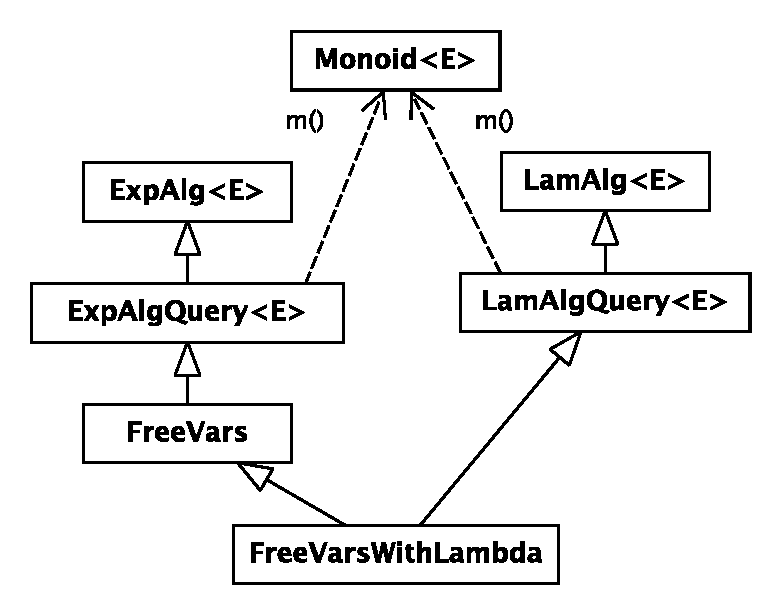
\includegraphics[width=0.9\linewidth]{extendQuery}
  \caption{Extension of the \lstinline{FreeVars} query}
  \label{FIG:extensionQuery}
\end{figure}


\begin{figure}[h]
  \centering
  \nocaptionrule
  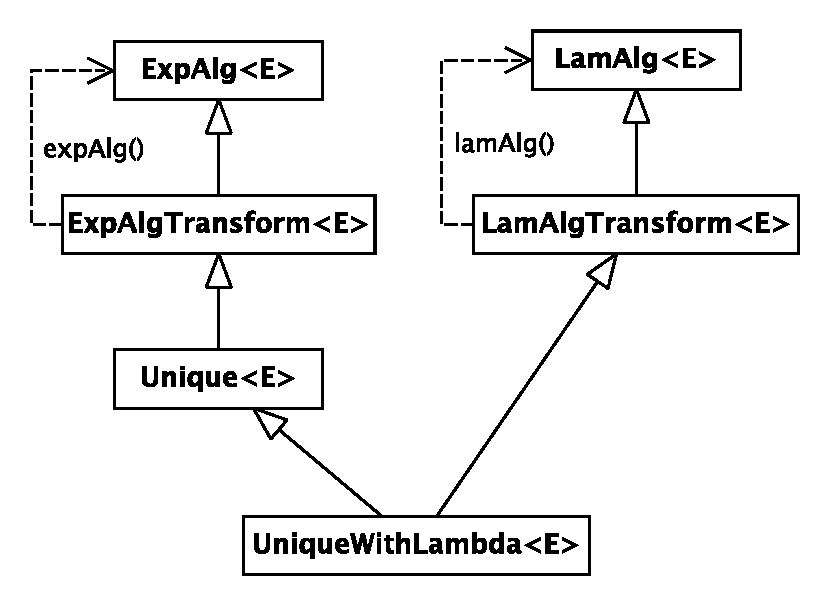
\includegraphics[width=0.9\linewidth]{extendTransform}
  \caption{Extension of the \lstinline{Unique} transformation}
  \label{FIG:extensionTrafo}
\end{figure}


Figures~\ref{FIG:extensionQuery} and~\ref{FIG:extensionTrafo} give a high level overview of query and transformation extension using the examples for \lstinline{FreeVars} and \lstinline{Unique}, respectively.
In the case of queries, the abstract \lstinline{m()} method will be shared by both the \lstinline{FreeVars} and \lstinline{FreeVarsWithLambda} interfaces.
On the other hand, transformations are based on multiple base algebras, for sets of data type constructors (e.g., \lstinline{expAlg()} and \lstinline{lamAlg()}).

Note finally that, in the current implementation of \name transformations, it is assumed that the language signatures \lstinline{ExpAlg} and \lstinline{LamAlg} are completely independent.
This is however, not an essential requirement.
An alternative design could have \lstinline{LamAlg} be a proper extension of \lstinline{ExpAlg} (i.e. \lstinline{LamAlg<E> extends ExpAlg<E>}).
In that case, the generated \lstinline{LamAlgTransform} would need to refine the return type of the \lstinline{expAlg()} method.


